% !TEX TS-program = PDfLaTeX
% !TEX encoding = UTF-8
%%
%% AUTORZY szablonu - proszę nie kasować tego komentarza
%Wykonali: Klaudia Olszewska, Natalia Smolińska, Oleksandra Koval, Krzysztof Bielas
%%
\documentclass[12pt,a4paper,oneside]{mwrep}
\usepackage[utf8]{inputenc}
\usepackage[T1]{fontenc}
\usepackage[polish]{babel}
\usepackage[unicode]{hyperref}	

\setlength{\parindent}{4pt}
\setlength{\parskip}{1ex plus 0.5ex minus 0.2ex}

					%W poniższych komentarzach (oznaczonych czerwonym kolorem) znajdują się instrukcje według,
                 					%których należy postępować. Sprowadzają się do wpisywania prostych danych.	
                     				%W nawiasy klamrowe są już wpisane przykładowe dane, które należy zmienić według własnego
\frenchspacing						%uznania.
\usepackage{indentfirst}										%POZOSTAŁEGO KODU NIE NALEŻY ZMIENIAĆ
\usepackage{graphicx, color}
\usepackage{tabularx}
\usepackage{colortbl}	
\usepackage[abs]{overpic}
\usepackage{xcolor,varwidth}
\usepackage{multirow}
\usepackage{caption}	
\usepackage[final]{pdfpages}
\usepackage{lipsum}
\usepackage{url}
\usepackage{float}



%%\usepackage{bookman}              %%  chcąc zmienić font, odkomentuj ta linię
\newcommand{\linia}{\rule{\linewidth}{0.5mm}}	
\makeatletter
\usepackage[top=2cm, bottom=2cm, left=3cm, right=2cm]{geometry}		
\renewcommand{\maketitle}{\begin{titlepage}

	\begin{center}
\huge{\textbf{WYŻSZA SZKOŁA ZARZĄDZANIA \\ ,,EDUKACJA"}}\\[2mm]
	\large {Wydział Zarządzania}\\
	\large {Kierunek:}
	\large												%W poniższy nawias klamrowy wpisz małym literami NAZWĘ KIERUNKU
	 															{informatyka}	
	\end{center}
	\vspace*{3cm}	
	\begin{center}
		\begin{minipage}{8cm}\textbf{}
		\centering
		\textit{}\\
		\Large \textsc{\@author} \\
		\Large {\textsc {Numer albumu:}
		\textsc										%W poniższy nawias klamrowy wpisz NUMER ALBUMU
																{24783}
		}
		\end{minipage}
	\end{center}
	\vspace{2cm}
	\begin{center}	
			\huge
		 	\MakeUppercase{\textbf{\textsc{\@title}}}\\
			\vspace*{0.2cm}
			\large \textbf {Praca} 		
			\MakeLowercase{\large \textbf						%W poniższy nawias klamrowy wpisz  co to jest za praca.
																{Inżynierska}
			}													
	\end{center}
				
	\vspace{3cm}	
	\begin{flushright}
	\begin{minipage}{8cm}
		\begin{flushleft}
		{\large Praca napisana \\ pod kierunkiem naukowym:}\\
		\vspace{0.3cm}
		\Large											%W poniższy nawias klamrowy wpisz tytuł,imię i nazwisko promotora.
																{dr inż. Piotr Grobelny}
		\end{flushleft}
	\end{minipage}	
	\end{flushright}
	\vspace*{\stretch{10}}
	\begin{center}
		%%\today
Wrocław 2019
	\end{center}	
\end{titlepage} %
}
\makeatother	
\author												%W poniższy nawias klamrowy wpisz imię i nazwisko autora.
																{Grzegorz Dzikowicki}
																
																
\title 													%W poniższy nawias klamrowy wpisz temat pracy.
														{Projekt gry komputerowej z wykorzystaniem silnika Unity}
%%
%%%%Rozdziały biegnące ciurkiem%%%%zakomentuj poniższe linie, jesli chcesz, aby rozdziały zaczynały się od nowej strony%%%%%
\SetSectionFormatting{chapter}
{48pt plus5pt minus2pt}
{\FormatHangHeading{\Large}}
{24pt plus3pt}
%%%%%%%%%%%%%%%%%%%Koniec macra Rozdziały biegnące ciurkiem%%%%%%%%%%%%%%%%%%%%%%%
%%
%%definicje własnych kolorów
\definecolor{kolor}{cmyk}{0.15,0.78,1,0.04}
\definecolor{kolor2}{cmyk}{0.15,0.78,1,0.09}
%%

\pretolerance=1000  %%% globalne ustawienie dzielenia wyrazów na końcu linii; wyższa wartość 'zabrania' dzielenia

\newenvironment{Table}
{\par\medskip\noindent\minipage{\linewidth}}
{\endminipage\par\medskip}
%%
\begin{document}
\maketitle
\baselineskip=19pt  %%%% odstępy międzywierszowe
%%
\tableofcontents
\newpage
\setcounter{page}{2}
\normalsize\rmfamily
\baselineskip24pt
%%
\chapter*{Wstęp}
%%
\begin{quotation}
\indent Gry komputerowe już od wielu lat kreują nowe trendy. Istnieją dwa różne rodzaje gier. 
Gry typu AAA tworzone przez wielkie studia gier jak np. Ubisoft, Electronic Arts, czy też nasz rodzimy CD Project Red. 
Patrząc na gry komputerowe klasy AAA możemy śmiało powiedzieć, że przypominają filmy rodem z Disney'a czy też Pixar'a. 
W dzisiejszych czasach aby oszczędzić sobie czasu, wiele dużych studiów używa technologii Motion Capture, aby odwzorować idealnie ruch postaci. Sprawia to,
że potrzeba manualnego rigowania postaci --- ustawienia ruchu postaci w sposób realistyczny --- przestaje być kłopotem grafików, oraz animatorów, którzy mogą skupić się na innych aspektach swoich zadań.

\indent Gry typu Indie są to produkcje które zazwyczaj są tworzone przez jedną osobę bądź amatorskie studio złożone z kilku osób. Ze względu na brak funduszy oraz wyposażenia studia, produkcje te zazwyczaj są niskiej jakości bądź średni czas potrzebny do przejścia gry jest o wiele krótszy niż gry AAA.
W dzisiejszych czasach jest pełno gier, których grafika składa się z pikseli, voxeli czyli sześciokątów oraz w stylu low-poly który zostanie wykorzystany do tego projektu.

\newpage 
\end{quotation}

%%
%%%
\chapter{Przegląd literatury}

w latach 60--tych XX~w. Departament Obrony Stanów Zjednoczonych rozpoczął tworzenie sieci komputerowej (ARPANET), której celem było połączenie uniwersytetów oraz innych jednostek realizujących projekty dla armii w~celu umożliwienia im wzajemnego dostępu do mocy obliczeniowej komputerów. Gdy w~późniejszym okresie opracowano rodzinę protokołów TCP/IP i~zaimplementowano je w~systemach UNIX’owych okazało się, że niemal natychmiast sieć ARPANET powiększyła się o~wszystkie lokalne sieci komputerowe zainstalowane w~uniwersytetach stanowych \cite{ss3,ss4,ss5}.

\lipsum[1-1]

\begin{quote}
\scriptsize{
\underline{\textcolor{blue}{Objaśnienie:}}\\[1mm]
\textcolor{blue}{\textbf{Przegląd literatury} (cz. teoretyczna objętość 10--15 str.)}\\[1mm]
\textcolor{blue}{
Rozdział podzielony na 2-4 podrozdziałów musi zawierać odpowiedzi na następujące pytania:
\begin{itemize}
\item  Jaka problematyka z~zakresu informatyki będzie analizowana?
\item  Jakie definicje, pojęcia będą wykorzystane w~pracy? (muszą być wyjaśnione słowa kluczowe zawarte w~tytule pracy)?
\item  Jak problem ewaluował historycznie? Co się zmieniało? Dlaczego? Co było tego przyczyną?
\item  Jacy autorzy (polscy, zagraniczni) zajmowali się w~przeszłości tą problematyką ?
\item  Jakie są poglądy poszczególnych autorów prac naukowych w~poruszanych kwestiach?
\item  Jakie teorie, „\emph{szkoły}" ~aktualnie obowiązują? Jakie ośrodki są wiodące?
\item  Jakie są podobieństwa i~różnice między autorami w~rozpatrywanej problematyce?
\item  Jakie jest stanowisko dyplomanta? Jakie przyjmuje definicje, twierdzenia? Mogą być przyjęte od konkretnych autorów, byleby to zaznaczyć w~tekście (w przypisach).
\end{itemize} }}
\end{quote}


%%
\chapter{Cel pracy, wymagania użytkownika, założenia, zakres i~tezy pracy}
%%
\section{Cel pracy}\label{cel}
%%
Celem pracy jest stworzenie projektu gry komputerowej za pomocą silnika Unity której grafika będzie reprezentowała styl graficzny ,,low-poly$"$.
%%

%%
\section{Wymagania użytkownika}
%%
Przez użytkownika (zamawiającego) zdefiniowane zostały następujące wymagania:
\begin{itemize}
\item gra musi być stworzona w środowisku Unity,
\item projekt musi być przedstawiony w formie 3D,
\item gra powinna posiadać świat przedstawiony w postaci low-poly.
\end{itemize}
%%
%%
%%
\section{Założenia}
%%
Przy realizacji projektu przyjęto następujące założenia:
\begin{itemize}
\item do projektu należy stworzyć modele 3D samochodu oraz przeszkód,
\item zaprogramować skryptów obsługujących przedsięwzięcie.
\end{itemize}
%%
%%
%%
\section{Zakres}
%%
Zakres pracy obejmował:
\begin{itemize}
\item elementy modeli ze względu na braki funduszy, zostaną stworzone w programie Blender,
\item pracę ograniczono jedynie do trzech krótkich poziomów, ze względu na aktualny stan projektu.
\end{itemize}
%%
%%
%%
\section{Teza pracy}
%%
Na podstawie przeglądu literatury dotyczącego zagadnienia przyjęto następujące tezy pracy:
\begin{itemize}
  \item do prawidłowego zrealizowania projektu wystarczające jest środowisko Unity oraz Blender.
\end{itemize}
%%
%%
\chapter{Badania własne}
\indent Proces badawczy to proces planowego, celowego wykorzystania uzyskanych informacji oraz własnej wiedzy. Celem głównym pracy jest próba stworzenia projektu świata przedstawionego w stylu graficznym low-poly. Głównym problemem jest skala. Zadecydowano więc, że projekt będzie przedstawiał trzy poziomy, w których gracz musi omijać przeszkody aby przejść na poziom wyżej.

%%
\section{Blender}
\indent Rozpoczynając pracę związaną z tworzeniem grafiki 3D, postanowiłem dowiedzieć się o możliwych programach do właśnie takich zadań. Z pośród najbardziej popularnych można wymienić Blendera, Autodesk Maya, Houdini oraz ZBrush. Jednym z kryteriów wyboru była cena zakupu programu. Oczywistym wyborem jest Blender, ponieważ jest on darmowym oprogramowaniem oraz posiada większość opcji z ww. programów. Modele wykorzystane w projekcie muszą być stworzone w stylu low-poly, oznacza to, że wymagania co do złożoności siatki obiektu pod względem topologii nie są wygórowane, wręcz muszą być zaniżone. 
%%
\section{Styl grafiki -- Low-poly}

\indent Low-poly jest określeniem siatki modelu 3D, który charakteryzuje się małą ilością wielokątów popularnie zwanych poligonami. Na przestrzeni lat, patrząc na początki gier komputerowych, dzisiejsze miano low-poly róźnie się diametralnie od swoich poprzedników z przed dwóch dekad, ze względu na o wiele większą ilość poligonów oraz technologię dzięki której tworzenie modeli 3D jest o wiele łatwiejsze, jednakże dalej odbiega od modeli które są nastawione na realizm. Wówczas obiekt zachowuje znajomom nam geometrię, jednakże nie posiada on idealnie gładkich krawędzi które odwzorcowałyby przedmiot w świecie rzeczywistym.

\begin{figure}[hbt!]
\setcaptionwidth{0.75\linewidth}
\centering
  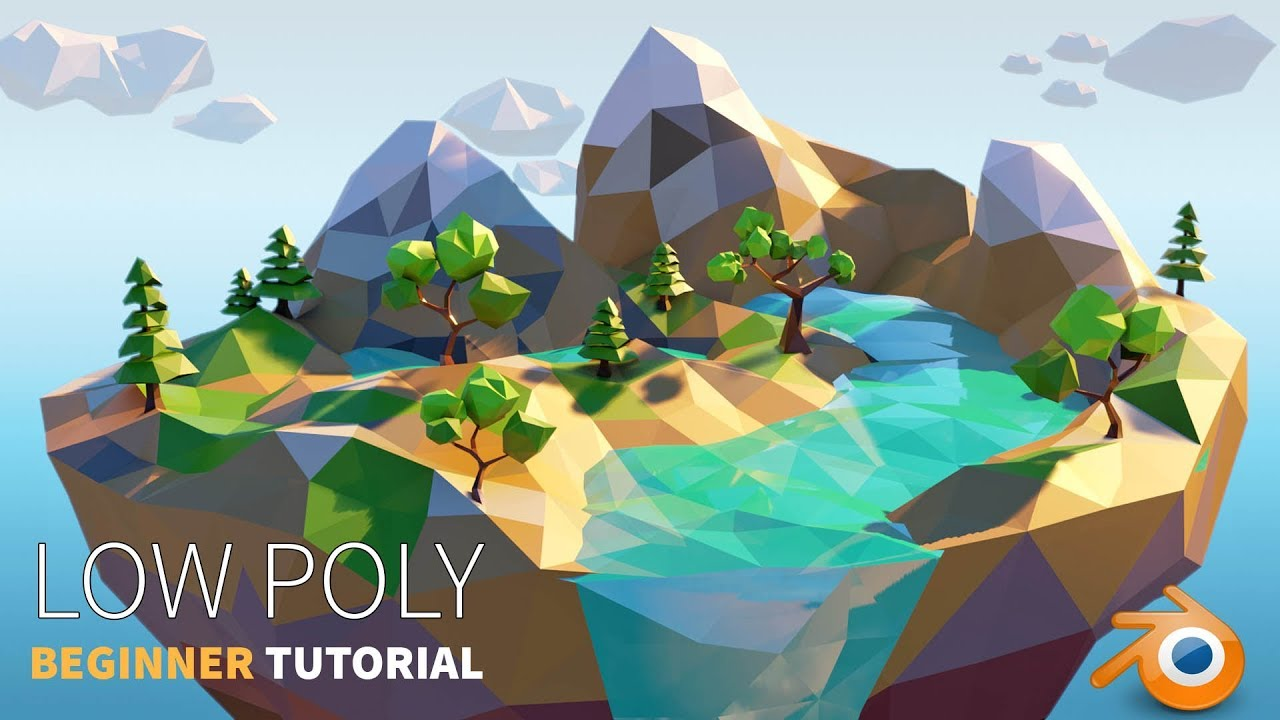
\includegraphics[width=0.75\linewidth]{lowpolytuto.jpg}
  \caption{Przykładowy render wyspy stworzonej w stylu low-poly}\label{rys_1}
  \begin{minipage}[t]{0.75\linewidth}
    \emph{Źródło: YouTube, CG Geek, Low Poly Island | Beginner | Blender 2.8 Tutorial, 2019.}
  \end{minipage}
\end{figure}

%%
\section{Unity}
\indent Istnieje wiele programów oraz silników do tworzenia gier komputerowych. Wiele dużych studiów takich jak Ubisoft, EA, CDProjektRED korzystają z własnych silników które sami napisali. Osoby, które tworzą gry w pojedynkę, korzystają z gotowych silników. Najpopularniejszymi są Unity oraz Unreal Engine. Wybierając Unity kierowałem się własnymi doświadczeniami związanymi z grami komputerowymi i programowaniem. Dużo gier, które miałem okazję zobaczyć było tworzone właśnie na silniku Unity. Unity pozwala programować w dwóch językach skryptów, C\# który jest podobny do C++, oraz JavaScript. C\# jest dla mnie bardzo intuicyjny ze względu na wielkie podobieństwo do C++ z którym miałem już doczynienia.
%%
\chapter{Metoda zrealizowania pracy}
%%
Realizacja pracy będzie się opierać na opracowaniu kroków, które należy podjąć aby stworzyć świat gry w stylu low-poly. Dodatkowo aby zaprezentować stworzone elementy, zostanie opracowane przedstawienie produktu za pomocą projektu gry komputerowej stworzonej w Unity.
%%
%%
\section{Narzędzia badawcze}
\begin{itemize}
\item Pierwszym narzędziem badawczym do stworzenia obiektów, będzie program Blender, który idealnie nadaje się do tworzenia elementów grafiki 3D,

\item drugim narzędziem badawczym, które posłuży do stworzenia gry komputerowej będzie środowisko Unity, w którym zostaną zaprogramowane podstawowe elementy rozgrywki,

\item trzecim narzędziem badawczym, dzięki któremu napiszemy kod do gry, będzie Microsoft Visual Studio 2017.

\end{itemize}
%%

\section{Technika tworzenia obiektów 3D}
\indent Obiekty grafiki 3D o mianie low-poly określa się przedmioty, postacie, świat gry itp. na których widać wyraźne elementy trisów bądź poligonów. Są to wyraźnie zaznaczone krawędzie obiektu, które swoją geometrią przypominają odpowiednik w świecie rzeczywistym, jednakże różnią się stopniem skomplikowania obiektu. Aby stworzyć taki model, najłatwiej jest zacząć od projektów poglądowych. W studiach gier, zazwyczaj zatrudnieni sią artyści, którzy podczas omawiania aspektów danych postaci bądź elementów świata, rysują proste szkice, które następnie poprawiają w celu uwydatnienia kluczowych aspektów obiektu. 
W późniejszym stadium rozwoju danego elementu, powstaje tzw. szkic końcowy. Wówczas owy szkic przekazuje się osobom, które zajmują się grafiką komputerową aby stworzyli dany obiekt w środowisku 3D. Do tego projektu użyłem zdjęć poglądowych dla beczki, oraz słupka drogowego.

\indent Tworząc obiekt zazwyczaj zaczyna się od zwykłej kostki sześciennej, którą następnie modyfikuje się, poprzez przesuwanie vertexów, krawędzi bądź całych ścian obiektu. Istnieje wiele narzędzi w Blenderze, które pomagają uzyskać porządany przez nas efekt takie jak Mirror. Dodając ten modyfikator na obiekt, otrzymujemy odbicie lustrzane ukazujące dwie identyczne połówki. Korzystając ze zdjęcia referencyjnego ustawionego w widoku side view (bocznym) możemy ustawiać krawędzie obiektu nadając mu identyczny kształt jak na zdjęciu. Samochód który będzie głównym pojazdem w projekcie został stworzony za pomocą zdjęcia poglądowego Poloneza oraz własnej wyobraźni, ponieważ jego proporcje oraz kształt są niczym wyjęte z kreskówki. Obiekty stworzone w Blenderze, zostały wyeksportowane jako plik typu fbx.

\begin{figure}[!h]
\setcaptionwidth{0.5\linewidth}
\centering
  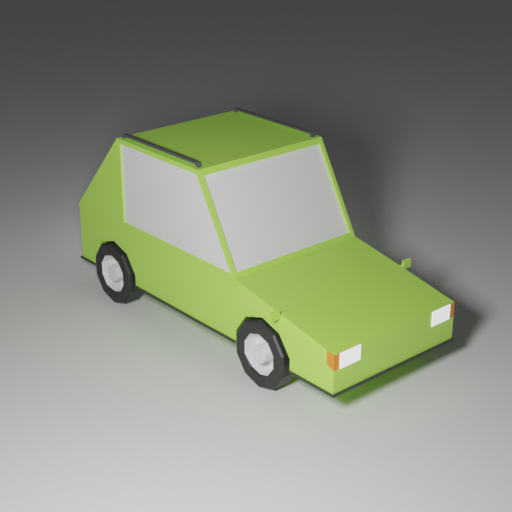
\includegraphics[width=0.5\linewidth]{carblend.png}
  \caption{Render samochodu stworzonego na potrzeby projektu}\label{rys_2}
  \begin{minipage}[t]{0.5\linewidth}
    \emph{Źródło: Grzegorz Dzikowicki}
  \end{minipage}
\end{figure}


\section{Środowisko Unity}
\indent Po wcześniejszym stworzeniu obiektów w Blenderze, przeszedłem do tworzenia środowiska w Unity. Aby obiekty nie wisiały w powietrzu, została stworzona płaska powierzchnia o rozmiarach 15x3x1000 jednostek Unity. Następnie umieściłem wszystkie obiekty w scenie. Każdy z obiektów posiada komponenty Mesh Collider, który odpowiada za wykrywanie kolizji z innymi obiektami, oraz Rigidbody będący głównym elementem fizyki obiektów.  Zostały zmodyfikowane ich masy oraz rozmiary aby stworzyć dla nich "prefab". Prefabem nazywany jest ten sam obiekt, jednakże po ponownym umieszczeniu go w scenie posiada te same właściwości. Ustawiając obiekty na powierzchni, stworzyłem 5 różnych poziomów, które różnią się trudnością, odpowiednio od pierwszego do piątego, bardziej skomplikowane ułożenie przeszkód oraz ich ilość. 

\indent Przejścia pomiędzy poziomami będą zawierały krótką i prostą animację wyświetlającą wiadomość "LEVEL COMPLETE". Tworzenie animacji polega na stworzeniu Panelu z tekstem a następnie na osi czasu zmiany wartości alfy, tak aby napis oraz tło pojawiły się. W sekcji programowania znajduje się kod, odpowiedzialny za proces przejścia z jednego poziomu na drugi. 

\section{Programowanie skryptów}
\indent Programowanie zacząłem od stworzenia skryptu obsługującego poruszanie się pojazdem. Aby obiekt się poruszał, wykorzystałem komponent Rigidbody umieszczony na samochodzie. Korzystając z gotowych funkcji zawartch w Rigidbody, mianowicie AddForce(), można sprawić aby obiekt poruszał się w danym kierunku z określoną mocą.

\begin{figure}[!h]
\setcaptionwidth{0.75\linewidth}
\centering
  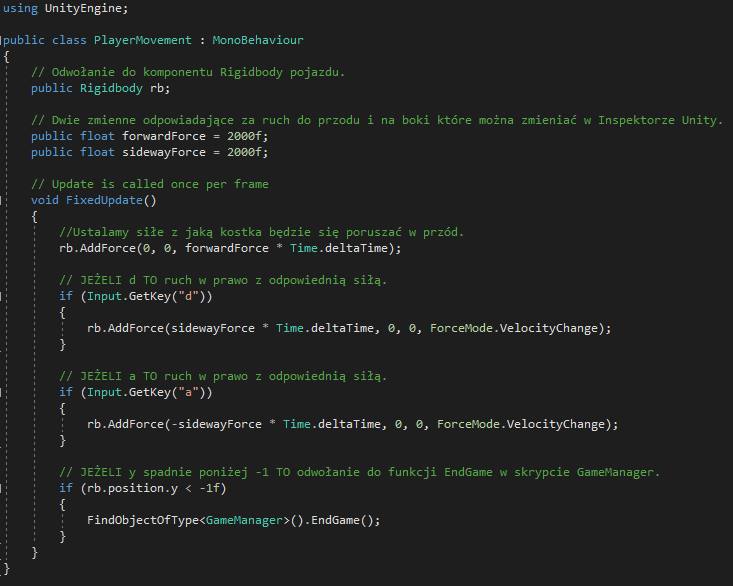
\includegraphics[width=1\linewidth]{playermove.png}
  \caption{Skrypt PlayerMovement obsługujący poruszanie się pojazdu po poziomie.}\label{rys_3}
  \begin{minipage}[t]{0.75\linewidth}
    \emph{Źródło: Grzegorz Dzikowicki}
  \end{minipage}
\end{figure}

\indent Kamera musi śledzić gracza, dlatego też napisałem skrypt, który ustala pozycję kamery w świecie gry, na taką samą pozycję co pojazd, jednakże dodawany jest offset, który podnosi kamerę do góry i przesuwa ją do tyłu, tak aby widok był z perspektywy trzeciej osoby.

\begin{figure}[!h]
\setcaptionwidth{0.75\linewidth}
\centering
  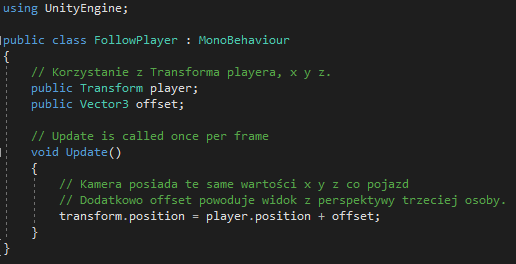
\includegraphics[width=1\linewidth]{followplayer.png}
  \caption{Skrypt FollowPlayer obsługujący umieszczenie kamery za pojazdem.}\label{rys_4}
  \begin{minipage}[t]{0.75\linewidth}
    \emph{Źródło: Grzegorz Dzikowicki}
  \end{minipage}
\end{figure}

\newpage
\indent Kolejnym przedsięwzięciem było napisanie skryptu, który będzie wykrywał kolizje z przeszkodami oraz resetował poziom, jeżeli pojazd spadnie z planszy. Ponieważ platforma po której porusza się pojazd, również jest wykrywana jako kolizja, wszystkie przeszkody zostały otagowane jako Obstacle. W skrypcie PlayerMovement został dodany kod obsługujący resetowanie poziomu, jeżeli wartość y pojazdu spadnie poniżej -1, który odwołuje się do funkcji EndGame w skrypcie GameManager.

\begin{figure}[!hbt]
\setcaptionwidth{0.75\linewidth}
\centering
  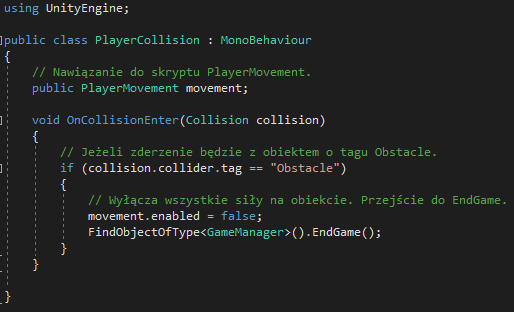
\includegraphics[width=1\linewidth]{playercollision.png}
  \caption{Skrypt PlayerCollision obsługujący kolizje pomiędzy pojazdem a przeszkodami.}\label{rys_5}
  \begin{minipage}[t]{0.75\linewidth}
    \emph{Źródło: Grzegorz Dzikowicki}
  \end{minipage}
\end{figure}
%%
\begin{figure}[!ht]
\setcaptionwidth{0.75\linewidth}
\centering
  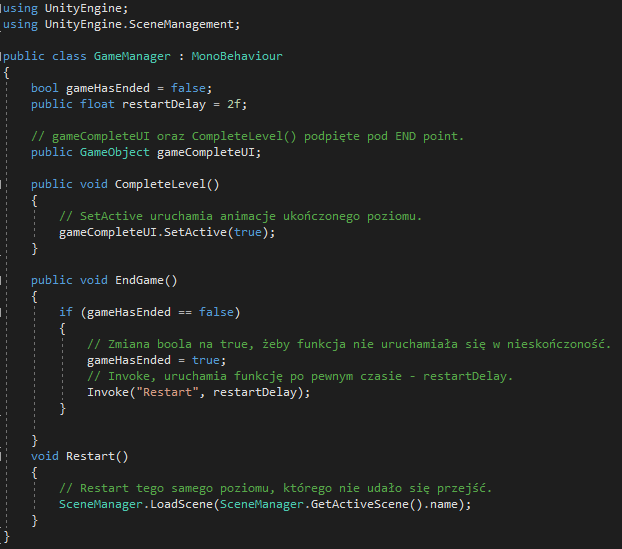
\includegraphics[width=1\linewidth]{gamemanager.png}
  \caption{Skrypt GameManager zajmujący się restowaniem poziomów.}\label{rys_6}
  \begin{minipage}[t]{0.75\linewidth}
    \emph{Źródło: Grzegorz Dzikowicki}
  \end{minipage}
\end{figure}

\indent Ponieważ w inspektorze nie da się podpiąć skryptu GameManager do prefabu pojazdu, w skrypcie PlayerCollision znajduje się metoda FindObjectOfType która przeszukuje w lokalizacji skryptów plik o nazwie GameManager a następnie korzysta z jego funkcji która musi być ustawiona jako public. Tworząc boola gameHasEnded, którego wartość zmieniana jest przy pierwszym uruchomieniu funkcji, upewniamy się, że funkcja będzie ładowana tylko jeden raz. Następnie po upadku, bądź kolizji, poziom jest ładowany od nowa, tak więc gameHasEnded ma swoją pierwotną wartość. Aby gra nie resetowała się za szybko, zamiast uruchamiać funkcję EndGame od razu, wykorzystałem metodę Invoke która po dodaniu nazwy funkcji, oraz czasu w sekundach, uruchamia funkcję po chwili. Aby przejść na następny poziom, musimy przejechać pomiędzy przeszkodami tak żeby ich nie dotknąć. W przypadku porażki poziom zostanie załadowany od nowa.

\indent Poziom jest już możliwy do przejścia, jednakże trzeba załadować kolejny. Na końcu trasy każdego z poziomów umieściłem kostkę o szerokości 15 jednostek Unity, która jest niewidoczna i służy jako Trigger, który uruchamia animację zakończonego poziomu, oraz ładuje kolejny. W skrypcie EndTrigger znajduje się jedna funkcja OnTriggerEnter(), która ładuje funkcję CompleteLevel() ze skryptu GameManager odpowiedzialną za włączenie animacji zakończenia poziomu.

\begin{figure}[!ht]
\setcaptionwidth{0.75\linewidth}
\centering
  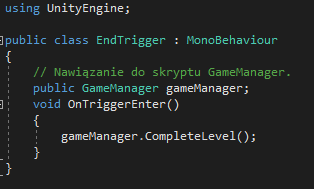
\includegraphics[width=1\linewidth]{endtrigger.png}
  \caption{Skrypt EndTrigger.}\label{rys_7}
  \begin{minipage}[t]{0.75\linewidth}
    \emph{Źródło: Grzegorz Dzikowicki}
  \end{minipage}
\end{figure}

\begin{figure}[!ht]
\setcaptionwidth{0.75\linewidth}
\centering
  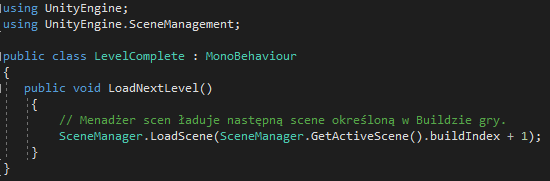
\includegraphics[width=1\linewidth]{loadlevel.png}
  \caption{Skrypt LevelComplete ładujący kolejny poziom.}\label{rys_8}
  \begin{minipage}[t]{0.75\linewidth}
    \emph{Źródło: Grzegorz Dzikowicki}
  \end{minipage}
\end{figure}

%%
%\input{wyniki.tex}
%\input{podsumowanie.tex}
%%
\chapter{Wnioski}
%%
Realizacja pracy pozwoliła sprecyzować następujące wnioski:
\begin{enumerate}
  \item do stworzenia gry 3D w stylu low poly wystarczające jest środowisko Unity,
  \item Blender jest wystarczająco dobrym środowiskiem do tworzenia obiektów 3D.
\end{enumerate}



\begin{quote}
\scriptsize{
\underline{\textcolor{blue}{Objaśnienie:}}\\[1mm]
\textcolor{blue}{{\textbf{Wnioski}:} (lista syntetycznych wniosków)}\\[1mm]
\textcolor{blue}{
Wnioski powinny:
\begin{enumerate}
\item jednoznacznie określać czy i~jak został osiągnięty cel pracy,
\item podsumować w~jaki sposób zweryfikowano hipotezy (jeśli były postawione),
\item odpowiadać na pytanie o~słuszność tez (czy je udowodniono).
\end{enumerate}
}}
\end{quote} 

\renewcommand{\bibname}{Spis literatury}
\nocite{*}
\bibliographystyle{unsrt}
\bibliography{biblio}
%\begin{quote}
%\scriptsize{
%\underline{\textcolor{blue}{Objaśnienie:}}\\[1mm]
%\textcolor{blue}{{\textbf{Literatura}:} (lista wszystkich przywołań i odwołań)}\\[1mm]
%\textcolor{blue}{
%Spis literatury, tzw. \emph{Bibliografia} powinna zawierać ponumerowany  wykaz - cytowanych w pracy, \textbf{w kolejności cytowania} - publikacji zwartych (książek), materiałów %konferencyjnych, artykułów w czasopismach naukowych, popularnonaukowych, źródeł elektronicznych (np. internetowych) itp. Stosować biblioteczną bazę danych BiB\TeX a oraz styl %cpm.bst.
%}}
%\end{quote}
\chapter*{Załączniki}
%%
\section{Zał. nr 1  Oświadczenie}
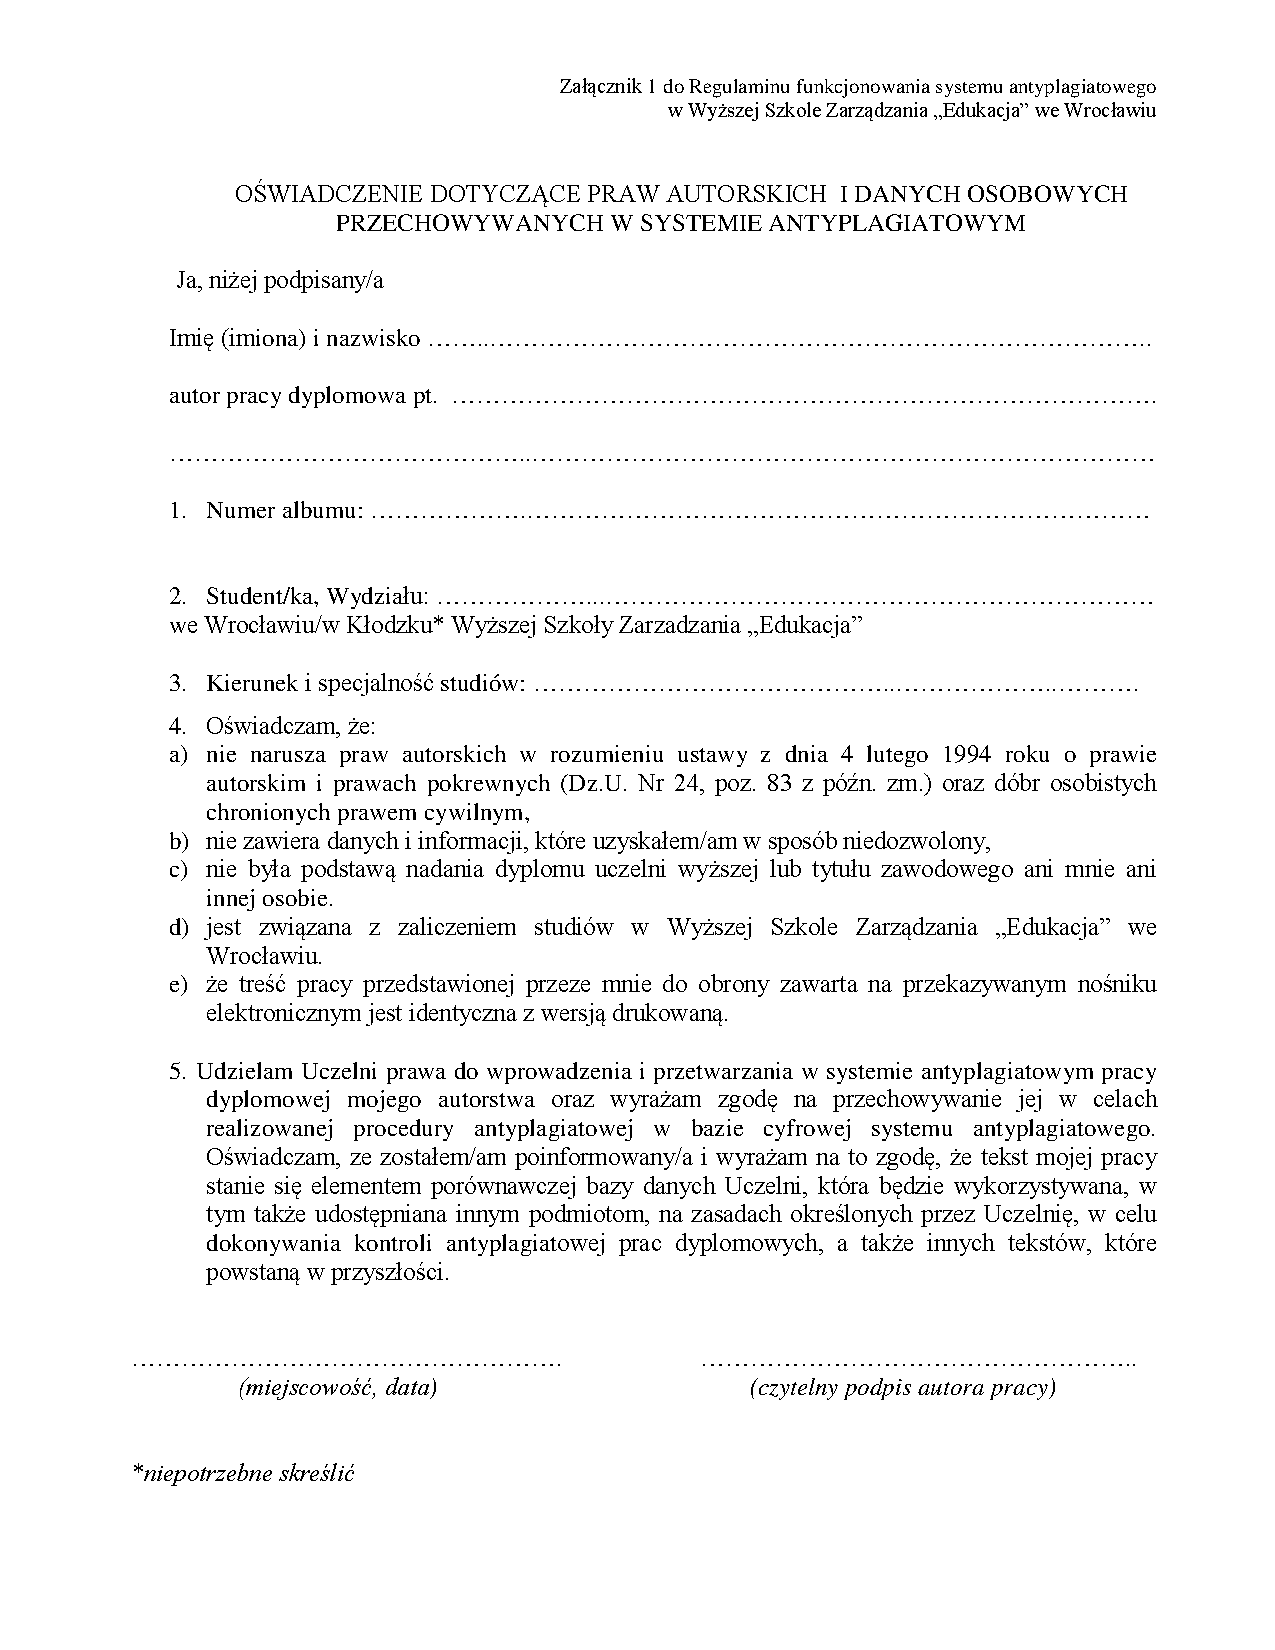
\includepdf[pages=-]{oswiadczenie.pdf}
%%%%
%%\section{Zał. nr 2 Dokument dziekanatu} %%
%%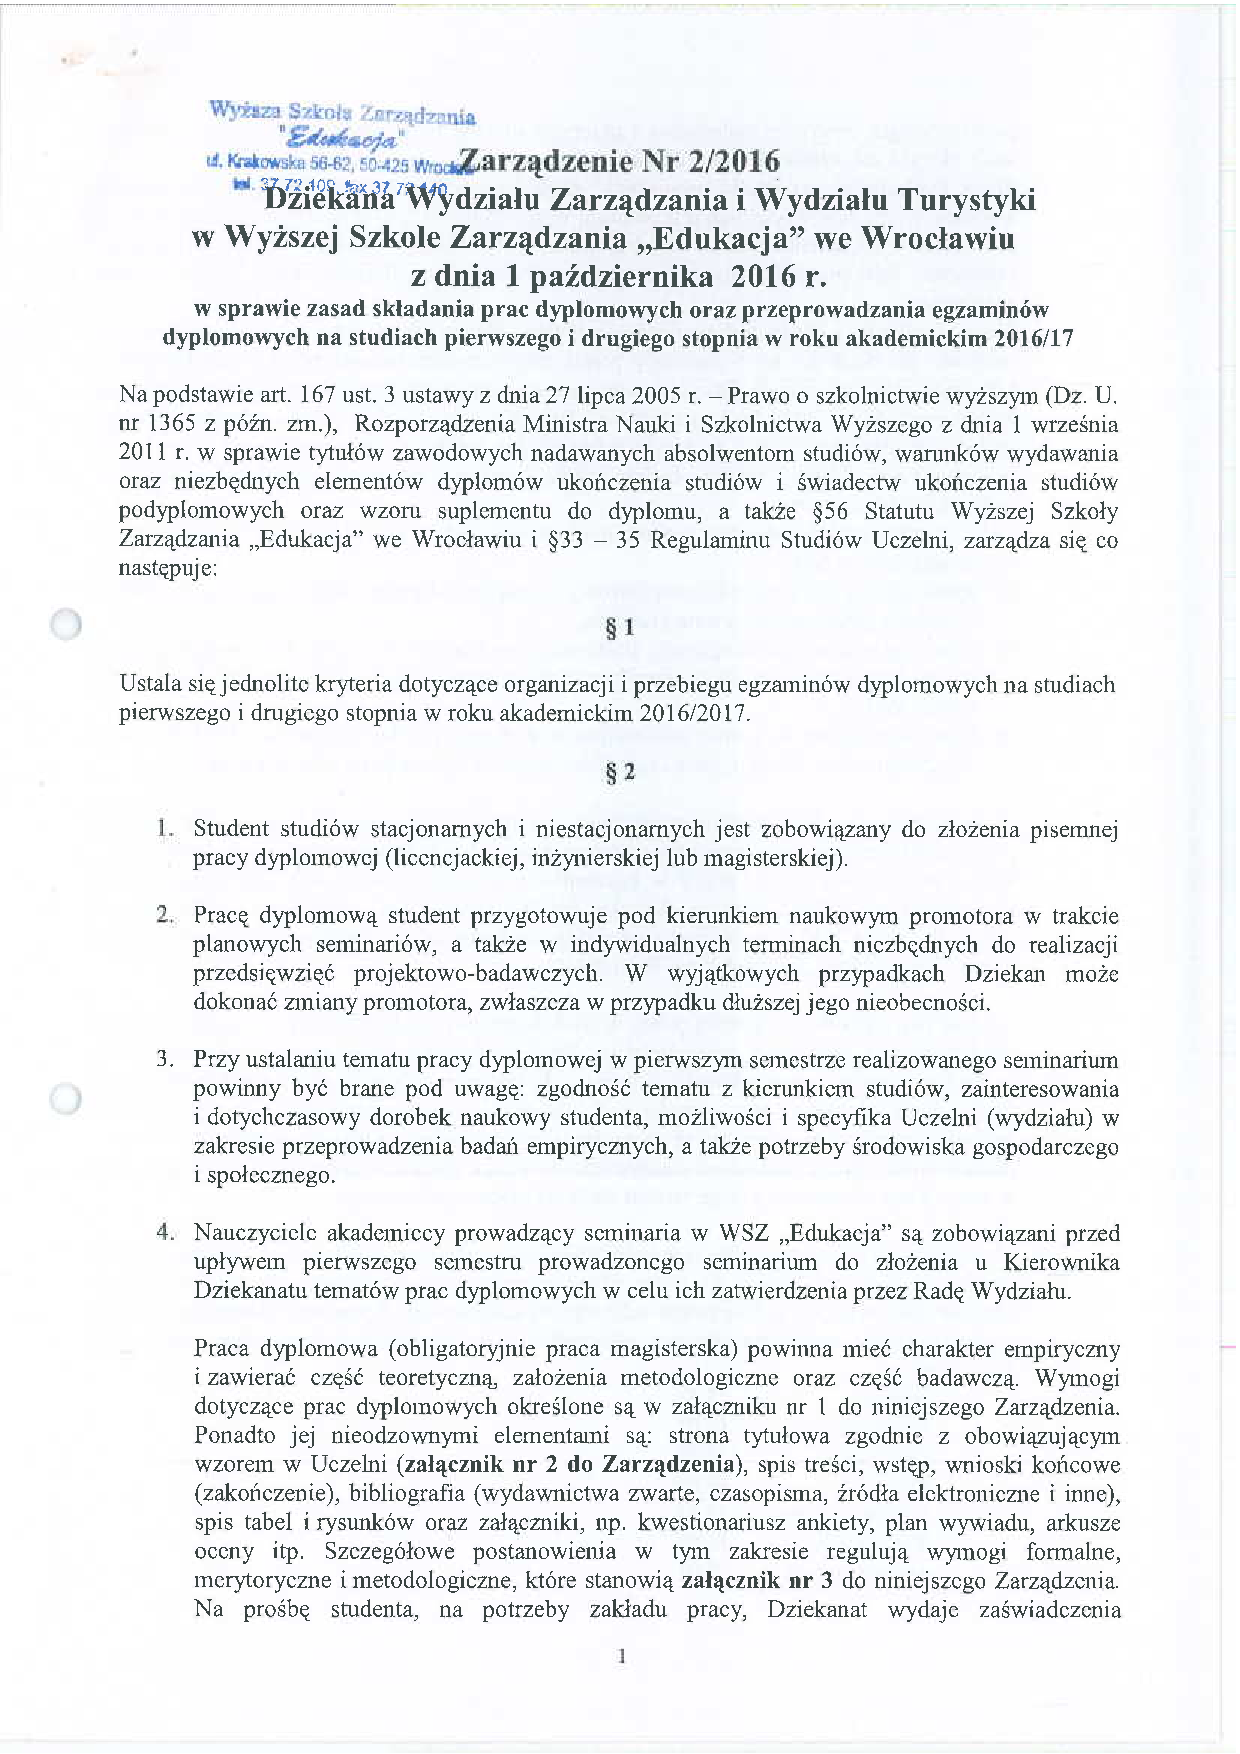
\includepdf[pages=-]{forma_pracy.pdf} 
%%
\end{document}
